
\Problem{Histogrames}

\Statement

Volem un programa per poder pintar histogrames com aquest:

\begin{center}
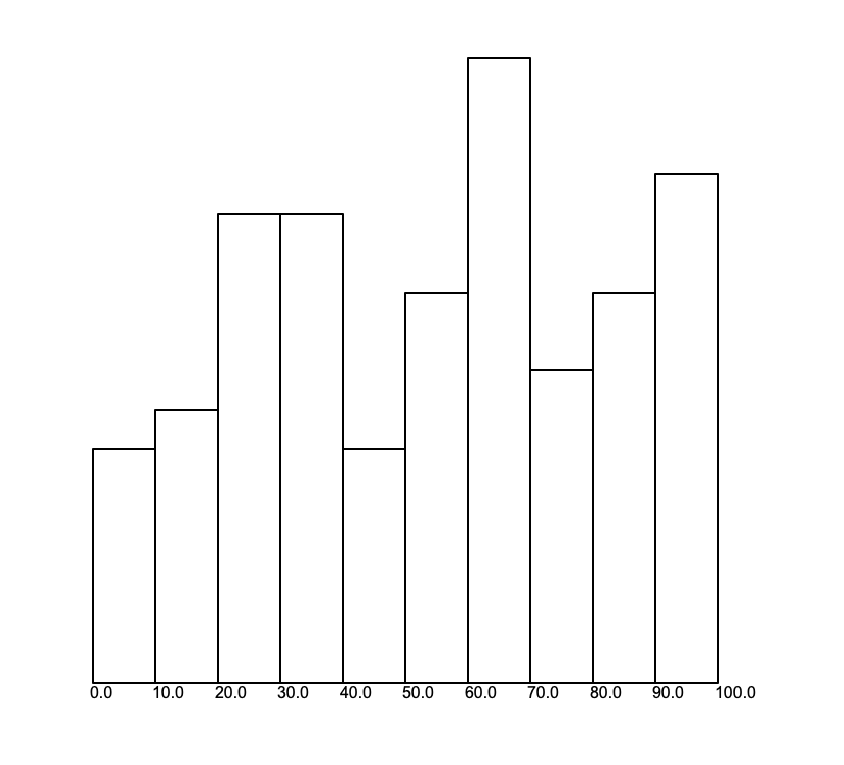
\includegraphics[height=6cm]{prova1.eps}
\end{center}


El programa ha de llegir primer un nombre natural que indica el nombre de barres desitjat. A continuació, el programa ha de llegir una seqüència (no buida) de nombres, tots positius. Finalment, el programa ha de dibuixar l'histograma, en una àrea de $300\times300$ píxels, tot escrivint els valors dels eixos de les $x$ on hi ha barres (amb un decimal). El valor a l'esquerra de l'histograma sempre ha de ser zero, el valor de la dreta ha de ser el màxim dels nombres donats. Totes les barres han de tenir la mateixa amplada, la barra més alta ha de tenir 300 píxels
d'alçada i l'alçada de les barres ha de ser proporcional al nombre d'elements
que representen.

\bigskip

Dibuixeu l'histograma amb el mòdul \texttt{turtle} de Python.
Les operacions que us poden caldre són
\texttt{forward},
\texttt{backward},
\texttt{right},
\texttt{left},
\texttt{goto},
\texttt{penup},
\texttt{pendown} i
\texttt{write}.
També, podeu usar \texttt{speed(0)} i \texttt{hideturtle()}
per accelerar la tortuga.
Per exemple, aquest programa pinta un quadrat amb un salutació al mig:

\begin{small}
\begin{verbatim}
import turtle

turtle.speed(0)
turtle.hideturtle()
for i in range(4):
    turtle.forward(300)
    turtle.left(90)
turtle.penup(); turtle.goto(150, 150); turtle.pendown()
turtle.write('Hola')
\end{verbatim}
\end{small}

\mysection{Observacions}

Aquest problema no té jocs de proves al Jutge. Per tant, qualsevol solució serà acceptada: semàfor verd! Això no vol dir que sigui bona ni dolenta, el vostre professor ho corregirà.

\medskip

Podeu convertir un real \texttt{x} a un text amb \texttt{str(x)} i podeu arrodonir
un real \texttt{x} a \texttt{k} decimals amb \texttt{round(x, k)}.



\clearpage

\begin{multicols}{2}\raggedcolumns
\mysection{Exemple d'entrada 1}

{\small
\begin{verbatim}
10

68 63 32 42 97 72 60 23 65 32 61
29 38 44 64 8 33 65 98 80 94 91
41 65 30 91 57 31 76 49 97 53 68
51 73 82 84 19 70 56 41 82 62 20
54 42 58 100 7 88 85 71 58 21 52
16 87 90 19 31 74 69 3 52 31 76
17 29 24 22 62 1 37 98 26 32 25
36 93 33 100 96 92 15 84 67 19
72 69 61 86 82 25 5 12 68 23 24
56 8
\end{verbatim}
}

\columnbreak

\mysection{Exemple de sortida 1}

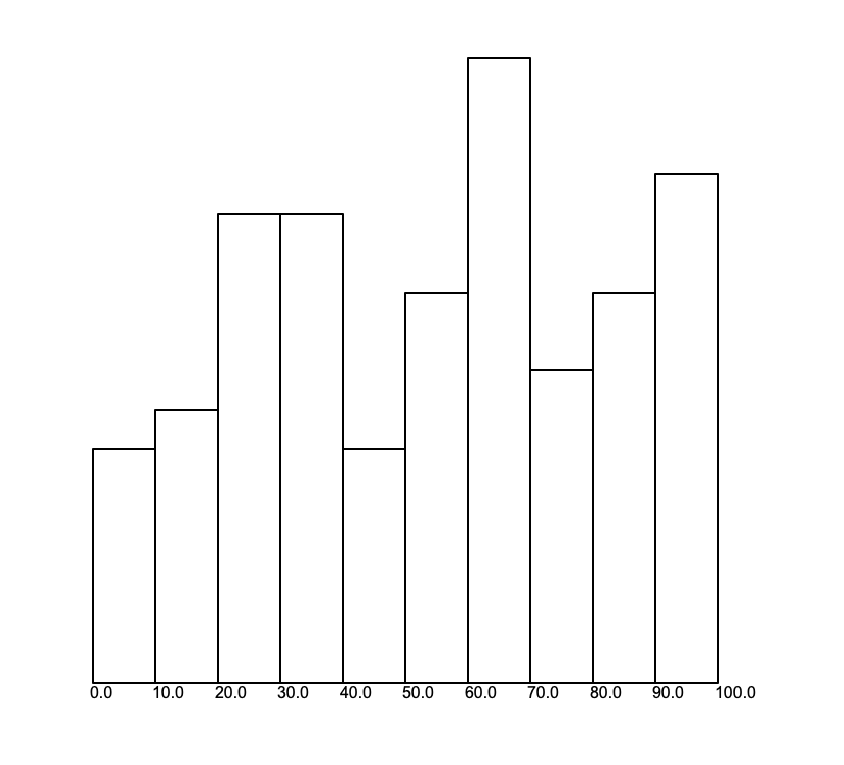
\includegraphics[height=5cm]{prova1.eps}

\end{multicols}



\begin{multicols}{2}\raggedcolumns

\mysection{Exemple d'entrada 2}

\begin{verbatim}
5

0 1 3 4
\end{verbatim}

\columnbreak

\mysection{Exemple de sortida 2}

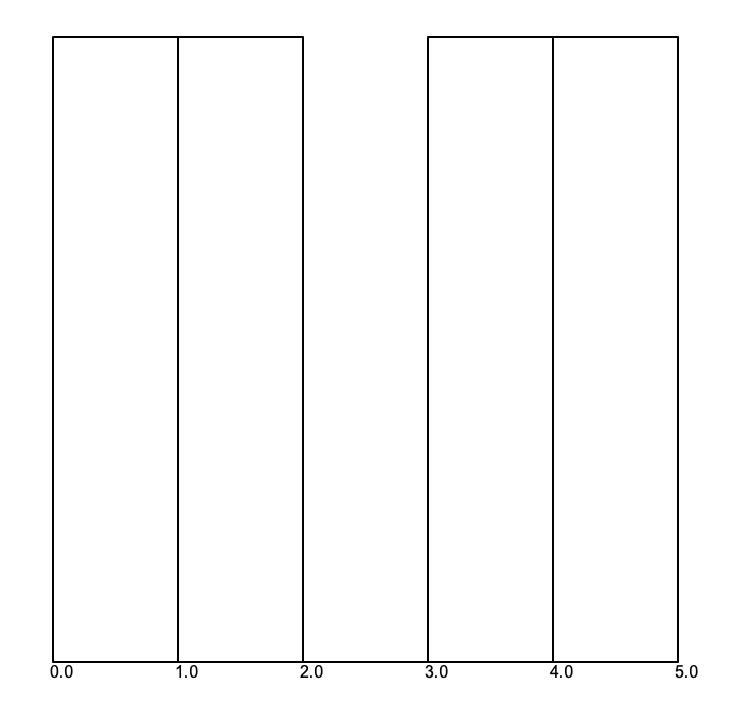
\includegraphics[height=5cm]{prova2.eps}

\end{multicols}



\begin{multicols}{2}\raggedcolumns

\mysection{Exemple d'entrada 3}

\begin{verbatim}
5

1 2 2 3 3 3 4 4 4 4
\end{verbatim}

\columnbreak

\mysection{Exemple de sortida 3}

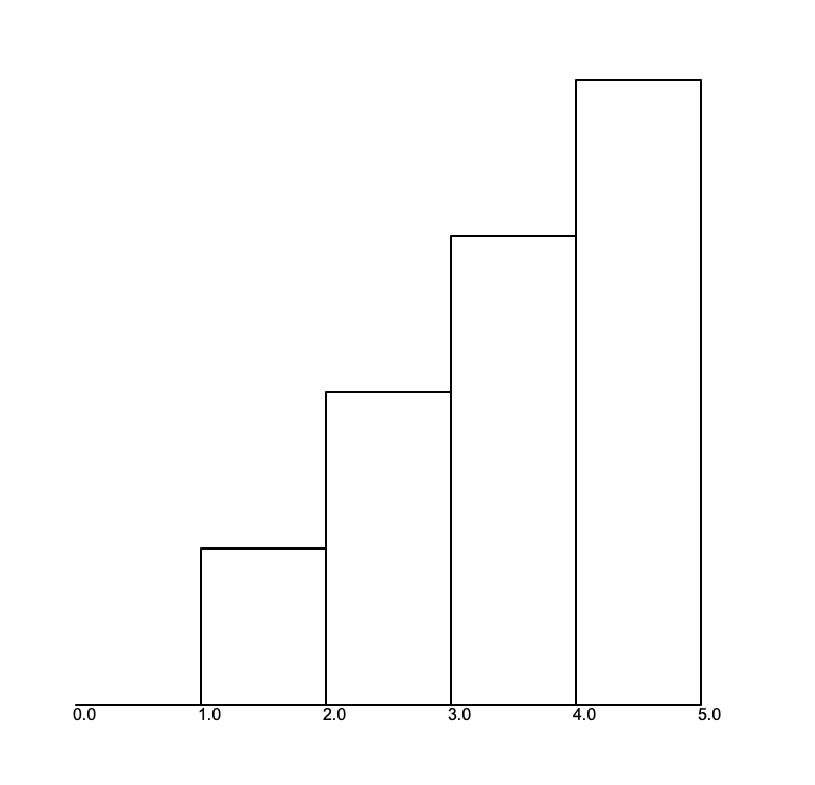
\includegraphics[height=5cm]{prova3.eps}

\end{multicols}


\begin{multicols}{2}\raggedcolumns

\mysection{Exemple d'entrada 4}

\begin{verbatim}
4

1 2 2 3 3 3 4 4 4 4
\end{verbatim}

\columnbreak

\mysection{Exemple de sortida 4}

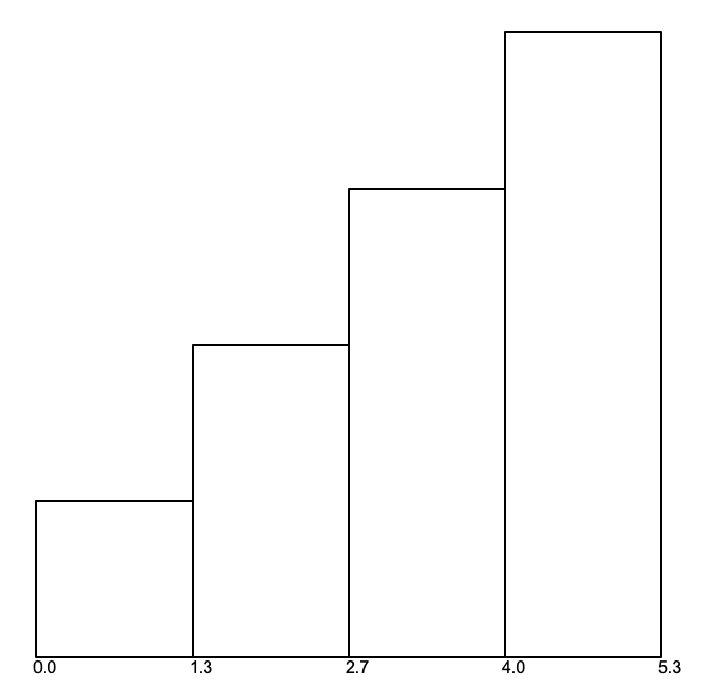
\includegraphics[height=5cm]{prova4.eps}

\end{multicols}
